\documentclass[12pt, a4paper]{article}

\usepackage[utf8]{inputenc} 
\usepackage[T5]{fontenc} 
\usepackage[vietnamese]{babel}
 
\usepackage[bottom = 1.5cm, top = 1.5cm, inner= 2cm, outer = 1.5cm]{geometry}

\usepackage{amssymb, amsthm}
\usepackage[intlimits]{mathtools}
\usepackage{graphicx}

\usepackage{float}
\usepackage{multicol}

%%%%%%%%%%%%%%%%%
\begin{document}

\title{Ứng dụng phổ $\gamma$ trong nghiên cứu cấu trúc hạt nhân $^{156}$GD}

\author{Đoàn Quang Tuyền\thanks{email: abc@gmail.com \newline tel: 0912345678}~, Nguyễn Văn A, Nguyễn Văn B\\
Viện nghiên cứu hạt nhân\\
\\
Nguyễn Văn C\\
Viện nghiên cứu hóa học}
\date{\relax}

\maketitle

\begin{abstract}
Tóm tắt nội dung của bài báo, nêu vấn đề, cách giải quyết vấn đề, các kết quả chính và kết luận, kiến nghị ..... 
\end{abstract}

\textbf{Từ khóa}: Cấu trúc hạt nhân, phổ gamma, ghi nhận bức xạ.

\begin{multicols}{2}

\section{Mở đầu}
\subsection{Cấu trúc hạt nhân}
Các mức năng lượng của hạt nhân được trình bày trên Hình \ref{fig:nangluong}...

\begin{figure}[H]
	\centering
	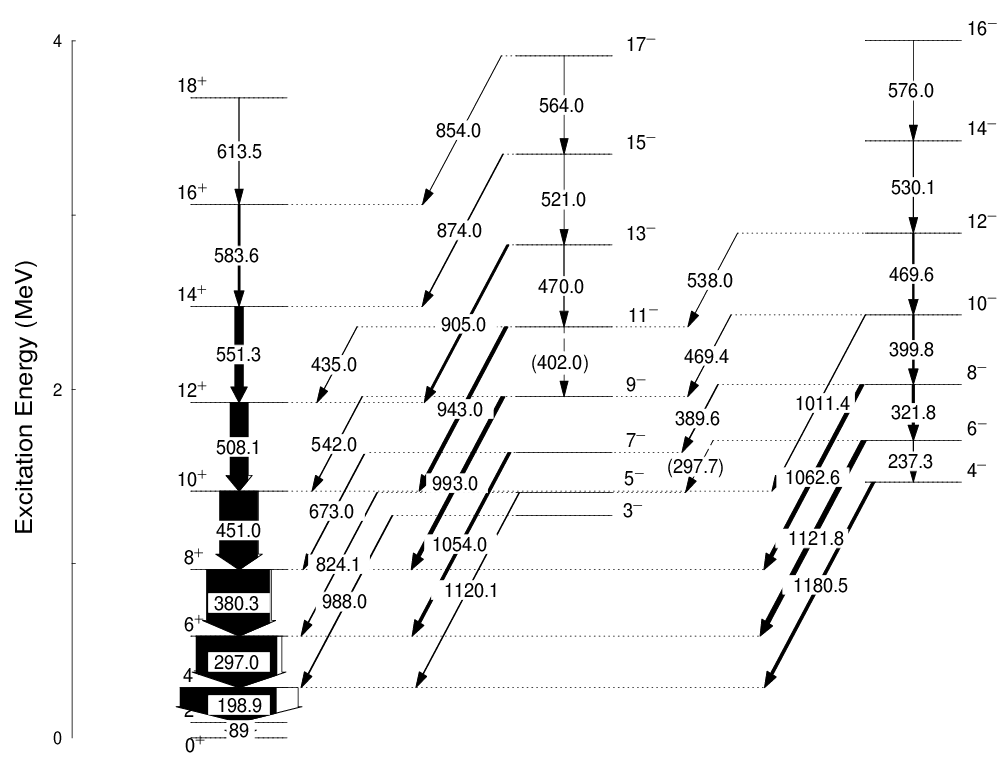
\includegraphics[width=0.7\linewidth]{156Gd.png}
	\caption{Mức năng lượng của hạt nhân.}
	\label{fig:nangluong}
\end{figure}

\subsection{Phổ $\gamma$}
Các phổ $\gamma$ đã được nghiên cứu trong các tài liệu \cite{bib_Bazzaco, bib_Simpson}

\section{Phương pháp thực nghiệm}
Trình bày các phương pháp thực nghiệm và sử lý số liệu ...

\section{Kết quả thực nghiệm}
Kết quả thực nghiệm được trình bày trên Bảng \ref{tab:solieu} ...
 
\begin{table}[H]
\centering
	\caption{Số liệu thực nghiệm.}
	\label{tab:solieu} 
	\begin{tabular}{ccc}
		\hline
		số tương tác	& Clover 	& Cluster\\
		\hline
		1	& 74.5 & 79.8\\
		2	& 22.4 & 18.3\\
		$\ge$3	& <3.3 & <2.8\\
		\hline
	\end{tabular}
\end{table}

\section{Kết luận}
Trình bày kết luận
\section{Lời cảm ơn}
Phần Lời cảm ơn ...

\bibliographystyle{ieeetr}
\bibliography{biblio}

\end{multicols}

\end{document}